
\begin{figure*}
	\center
	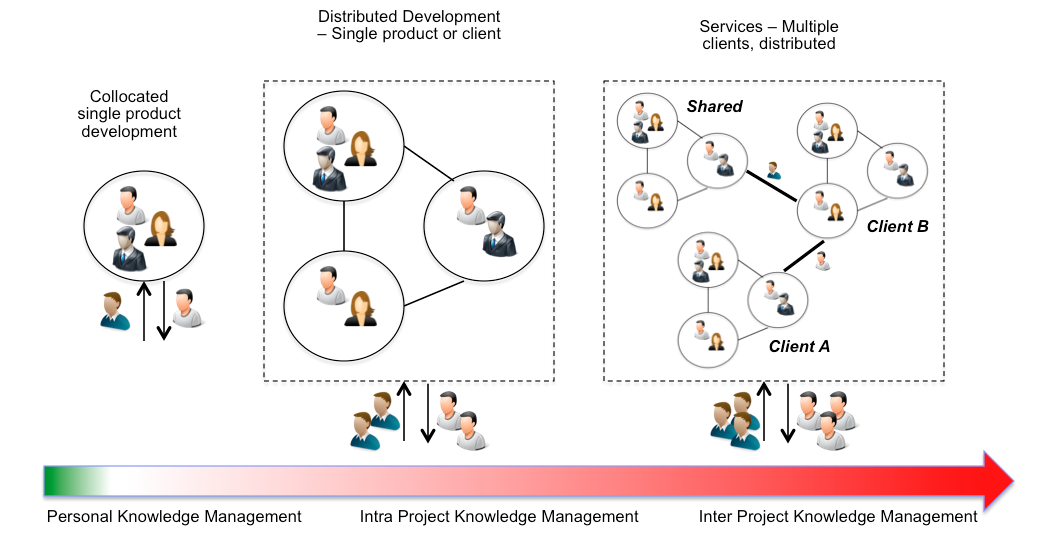
\includegraphics[scale=0.45]{figs/km-types.png}
	\caption{Team structures and knowledge management needs}
	\label{fig-km}
\end{figure*}

\section{Knowledge Management}
\label{sec:km}

Software development is inherently a knowledge intensive activity. Software designers and developers leverage their software development skills along with knowledge about the domain, past experiences and knowledge of team members, to solve the current problem at hand, be it implementing a new feature/application or solving a bug. Individuals are adept at managing their own knowledge and drawing upon it when a new situation comes in \cite{Bruce:2005}. For example, a developer who has been assigned a bug on a system (s)he has implemented would typically know where to start investigation from because of prior knowledge about the system. A project manager working long enough in the product would know the primary risks associated with the project, fault prone areas and so on. In small, colocated teams too, knowledge management is not a big challenge. Who is an expert on what part of the system is typically known. New team members coming in would use informal channels of communication to figure out who are the experts on the system. If need be, individuals can tap into the knowledge of these experts to quickly address task at hand. 

Knowledge management starts to become a challenge when team size increases and/or teams start getting distributed geographically. In large teams or distributed environments, the requisite knowledge of the system---expertise, best practices, insights, ideas and so on---is spread across multiple people, locations and even organizations (in cases such as outsourcing) \cite{Desouza:2006}. In such scenario, even for a single project a formal knowledge management system needs to be in place that stores all data for a project---be it requirements, assumptions, solution documents, design rationale, bugs, code artifacts and so on. Any project member should be able to refer to this project database to understand how project evolved, who are the experts in the system and given a task at hand search for relevant artifacts and activites from past. Now consider the case for services organizations such as IBM, which are developing and managing software systems for multiple clients. Information on how a requirement to develop a payroll system for client A could be applicable for another client B also. Knowledge of how a leave related issue implemented on SAP HCM was resolved for client C, could we leverage when solving a similar issue for client D. 
A cross-projects/cross-clients knowledge repository is like the organization memory \cite{Stein:1995} for services organizations and provides oppurtunities to leverage learnings from the past to achieve greater efficiency and efficacy in present and future projects. Figure~\ref{fig-km} illustrates how knowledge management needs in services organizations, evolve from personal knowledge management to intra-project and inter-project KM due to increased team sizes, geographic distribution and multiple client engagements. 

The rest of this section is organized as follows. We first describe why knowledge management is needed in services organizations, followed by design considerations for building an effective knowledge management system. Finally, we present our experiences with deploying two knowledge management systems within IBM.

\subsection{Need}

\begin{itemize}
\item Do things faster
\item Do things with less skilled resources
\item Handle resource churn
\item Promote reuse across engagements
\end{itemize}

\subsection{Design Considerations for Effective Knowledge Management}

\begin{itemize}
\item How and what to harvest: personalization versus codification, manually curated versus auto-harvested
\item Features needed from KM system: search, topics, summarization
\item How to promote usage: incentives, quality versus quantity
\end{itemize}

\subsection{Examples}
\begin{itemize}
\item Consultant's Assistant - KM at solution level
\item Wisdom - KM for troubleshooting
\end{itemize}
